\part{Seminar 9 - Dynamical Modelling of Passively Levitated Electrodynamic}

\makebox[.25\textwidth]{Damon Coates}\makebox[.25\textwidth]{Jeroen Domisse}\makebox[.25\textwidth]{Louis Fichefet}\makebox[.25\textwidth]{Thomas Lampe}

\section{Introduction}
Le titre du papier est "Dynamical Modelling of Passively Levitated Electrodynamic Thrust Self-Bearing Machines", on va déjà disséquer ce titre pour mettre en contexte :
\begin{itemize}
    \item Dynamical modelling : cela correspond à une approche différente, mais complémentaires des approches locales vues dans les autres séminaires. Jusque là nous avons principalement effectuer des modélisations locales en résolvant les équations de Maxwell et effectuant des éléments finis. Ici, on va appréhender le comportement de la machine de manière dynamique, tout en se servant d'approche locale là où c'est nécessaire (par exemple, dans la détermination des équations de fluxs)
    \item Passively Levitated Electrodynamic Thrust : la machine gènère une butée (autrement dit, gère son degré de liberté axial) electrodynamiquement. Le "passively" indique que cette butée n'est dû qu'à des phénomènes passifs
    \item Self Bearing : la machine génère sa propre butée (autrement dit, elle génère elle même sa stabilité axiale
\end{itemize}

On peut grossièrement dire que l'on a un rotor qui en tournant va induire des courants passifs qui lui permettront de léviter.

\section{Contexte}
Toute pièce de machine a 6 degrés de liberté. Via des palliers, on va chercher à contraindre 4 ou 5 de ces degrés de liberté pour que la pièce du rotor ne puisse plus que tourner selon un seul axe. Différents types de palliers existent : mécanique, magnétique (passif ou actif), bearingless. Leurs avantages et désavantages respectifs sont représentés dans la Table \ref{tab:Bearings}.

\begin{table}[H]
    \centering
    \begin{tabular}{|p{3cm}|p{5cm}|p{5cm}|}
    \hline
        Types de palliers & Avantages & D\'esavantages \\
        \hline
        \hline
        Mécanique & Super stable, facile à produire  & Frottement : ce qui cause de l'usure et empêche d'atteindre de très haute vitesse. Ils doivent être lubrifiés avec de l'huile (ce qui peut être un problème pour des procédés chimiques, pharmaceutiques) \\
        \hline
        Magnétique Passifs & Compact et plus fiable. Ces dernier se basant sur des phénomènes passifs, on est sur qu'ils se comportent toujours de la même manière 
        & Le Théorème d'Earnshaw interdit de stabiliser 6 degrés de libertés en utilisant que des champs magnétiques statiques 
        \\
        \hline
        Magnétique Actifs & L'\'electronique pr\'esente permet plus de contrôle et d'assurer la stabilité de 6 degrés de libertés. La constante de raideur peut aussi être ajustée à de plus grandes valeurs  & L'électronique présente prends plus de place, augmente le cout. \\
        \hline
        ``Bearingless'' : combiner la fonction motrice et de pallier & Plus compact et permet d'augmenter la vitesse  &  .\\
        \hline
    \end{tabular}
    \caption{Résumé des différents types de palliers, pour machines tournantes, avec leurs avantages et désavantages}
    \label{tab:Bearings}
\end{table}

Pour certaines applications (spatiales par exemple), on cherche à développer des machines tournantes :
\begin{itemize}
    \item Stable pour 5 degrés de liberté
    \item A faible coût
    \item Fiable 
    \item Qui peuvent atteindre de grandes vitesses de rotations
\end{itemize}

Ces critères pointent vers une solution magnétique passive "bearingless". Cependant, le théorème d'Earnshaw (expliqué en annexe) interdit de stabiliser 5 degrés de libertés avec uniquement des champs statiques. Il faut donc stabiliser au moins un degré de liberté différemment : ce sera fait électrodynamiquement à travers des phénomènes passifs.



\section{Equations de Flux} 
A la base du fonctionnement de ces machines se trouvent les flux. Donc avant d'expliquer comment fonctionne la machine, on va démontrer comment trouver les équations du flux. 
Notez ici, que on utilise bien une approche local de modélisation pour les flux. 



\section{Principe de fonctionnement}
La topologie étudiée représente N phases, p paire de pôles, avec z=0 comme position nominale. Sur la figure \ref{fig:topo}, on a 1 phase et 3 paires de pôles.

\begin{figure}
    \centering
    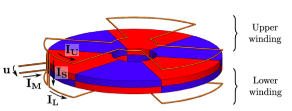
\includegraphics[scale=0.5]{Damon/Topologie.png}
    \caption{Topologie étudiée. Le rotor est fait d'aimants permanents, on observe qu'il y a des bobinages au dessus et en dessous.}
    \label{fig:topo}
\end{figure}

Les champs des aimants permanents au dessus et en dessous sont de directions différentes. Ainsi, en position nominale (z=0), le flux total intercepté par les enroulements est nul.
Lorsque z est différent de 0, ce flux total n'est plus nul et va induire un courant dans les enroulements. On vous renvoit aux slides 25 à 30 pour regarder la petite animation en mode diaporama : les courants passifs permettant de stabiliser le rotor apparaissent uniquement si le rotor n'est pas à sa position nominale (z=0)


Ce courant induit lui-même un champ magnétique qui en interagissant avec le champ des aimants permanents, va induire deux forces :
\begin{itemize}
    \item Une "restoring force" dans l'axe, dans la direction qui ramène le rotor vers sa position nominale
    \item Un "drag torque" qui vient s'opposer à la rotation\footnote{Pourquoi cette force s'oppose à la rotation ? Pensez à la conservation d'énergie. Si une force vient ramener le rotor vers sa position nominale, c'est grâce au courant induits dans les enroulements. Ces courants sont induits par la variation de flux, qui vient de la rotation (Voir Slide 53 à 56).}
\end{itemize}

\section{Trouver le flux intercepté par les enroulements}
Cette partie est la seule analyse "locale", comparée à l'analyse "globale" qui est faite à travers tout le séminaire (comme l'analyse par la théorie des circuits etc...). Les équations sont justes ignobles et ne nécessitent pas d'être apprises. La démarche est par contre intéressante et mérite d'être connue. Sachant qu'on a 3 repères différents en coordonnées polaires pour exprimer le stator(armature ou PM), le rotor (PM ou armature), et le rotor vu du stator, on doit :
\begin{enumerate}
    \item Dire que le champ $B(r,\theta,z)$ induit par les PMs est de forme :
    $$ B(r,\theta,z) = \cos(p\theta)f(z)g(r) $$
    Ce qui veut dire qu'il est fonction de la fondamentale du champ (le $\cos(p\theta)$) et "du reste" (sisi, c'est sérieux, c'est comme ça dans le papier).
    \item Exprimer les coordonnées des PMs ($r,\theta,z$) dans le repère de l'armature ($\xi,\psi,a$) via une cinématique inverse.
    \item Faire une approximation de Taylor de cette dernière expression (valide, car on considère les petits déplacements uniquement).
    \item Intégrer le champ magnétique sur la surface des enroulements pour obtenir le flux capté par une phase
    \item Simplifier grâce à des propriétés trigonométriques.
\end{enumerate}
Le résultat est que le flux intercepté par une phase est égal à :
$$ \Phi_k = (\Phi_0 + zK_{\phi})*\cos(p(\theta - \delta_k)) $$
avec $\delta_k$ égal à 0, 120 et 240\degree pour un système triphasé. Ici, il est important de noter que le flux varie linéairement avec la hauteur z, et que les constantes $\Phi_0$ et $K_{\phi}$ sont FORTEMENT dépendantes de la géométrie.\\
Notons aussi que pour augmenter le flux intercepté par les enroulements, on peut jouer sur deux paramètres :
\begin{itemize}
    \item Soit on joue sur la surface disponible (le $S$ de $\int_S B \dot n \ dS$), ce qui n'est pas possible dans le cas de l'EDTSB axial car la surface vue par les enroulements reste la même, mais dans le cas d'un EDTSB radial, oui !
    \item Soit on joue sur l'intensité du champ $B$ qui peut varier avec la distance entre les PMs et les enroulements (ce qui est possible avec le flux axial et radial). Une autre manière d'influer sur le champ $B$ est la présence de pièces ferromagnétiques, qui vont alors concentrer le champ.
\end{itemize}

\section{Simplification des équations avec la transformée de Park}
Le transformée de Park (ou la transformée dq0) est utilisée sur les équations électriques, parce ce qu'elle possède de nombreux avantages pour le contrôle es machines tournantes ; En effet, elles permettent, après une série de 3 rotations élémentaires, de fixer un repère sur le rotor, axé de telle manière qu'une des composantes (l'homopolaire ou composante 0) soit nulle dans le cas d'un steady-state. Les deux autres vecteurs sont appelés composante directe (d) et composante en quadrature (q).
\begin{figure}
    \centering
    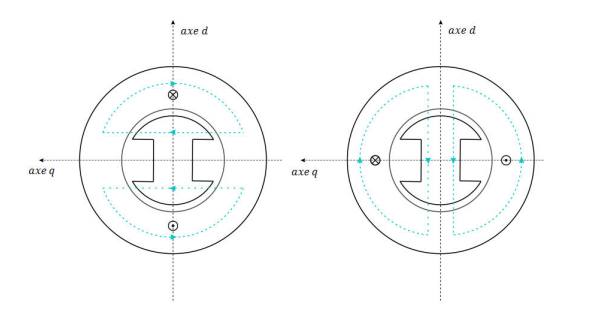
\includegraphics[width=\textwidth]{TRANSFORMEE.PNG}
    \caption{Interprétation des composantes d et q}
    \label{fig:dqo}
\end{figure}
La Figure \ref{fig:dqo} interprète très bien les deux composantes. La composante directe (d, à droite sur la Figure) va créer un champ magnétique qui sera axé avec la position du rotor. celui-ci va donc subir une \textbf{force}, dû à cet alignement. La composante en quadrature (q, à gauche sur la Figure) quant à elle, va forcer le rotor à tourner pour s'aligner avec le champ magnétique, ce qui va créer un couple.\\
Il est important de noter donc plusieurs choses : 
\begin{itemize}
    \item En steady-state, les inputs de courant dans la transformée dqo sont CONSTANTS (du DC donc), ce qui induit aussi que le contrôle des machines tournantes s'en trouve grandement facilité, car devoir répondre à une consigne de type \textit{step} ou \textit{ramp} est bien plus facile qu'une consigne sinusoïdale.
    \item Les équations sont grandement épurées de manière générale : plus de dépendance envers $\theta$ (mais une dépendance envers $\omega = \frac{d\theta}{dt}$ ce qui est préférable), les inductances deviennent constantes etc...
    \item La transformée de Park peut se faire sur un système N-phases avec $N=1,2,3...$ Dans ce cas, il faut utiliser la transformée généralisée, qui fait appel à des transformations complexes et devient plus compliquée, mais la finalité reste la même ! Sachez juste que c'est possible et que ça fait appel aux nombres complexes.
\end{itemize}
La transformée est donc utilisée pour réduire les équations électriques à leur plus simple apparat :) Il faut retenir de ça que, tout d'abord, en isolant la force $F_z$, on peut voir qu'elle est fonction du courant $I_{S,d}$. Et que le couple total est séparé en deux : couple moteur (fonction de $I_{M,q})$ et le couple résistant (fonction de $I_{S,q})$.\\
Si, dans ce dernier paragraphe, les dépendances aux courant vous semblent parfaitement normal/logique alors je vous dis bravo, car vous avez compris tout ce qu'il fallait comprendre là-dessus.

\section{Linéarisation}
A titre indicatif, je mets le numéro du slide pour un peu voir où on est dans la présentation. Normalement la synthèse peut être étudiée sans les slides! :)
\paragraph{Slide 66}

Ici c'est important de remarquer que le système (Figure \ref{fig:S66}) qu'on a obtenu n'est pas linéaire. Cependant, pour étudier la stabilité du système(objectif de cette partie), il faut linéariser pour pouvoir utiliser le root locus. Finalement si vous vous demandez d'où vient le système, c'est juste de l'algèbre des équations venant de la partie du modèle dynamique ( Slide 59 de la présentation ou dans le doc, ça vient des équations 22 , 26, 28, 29 et 30 mais c'est très long à faire et à notre sens ça sert à rien de le faire).
\begin{figure}[H]
    \centering
    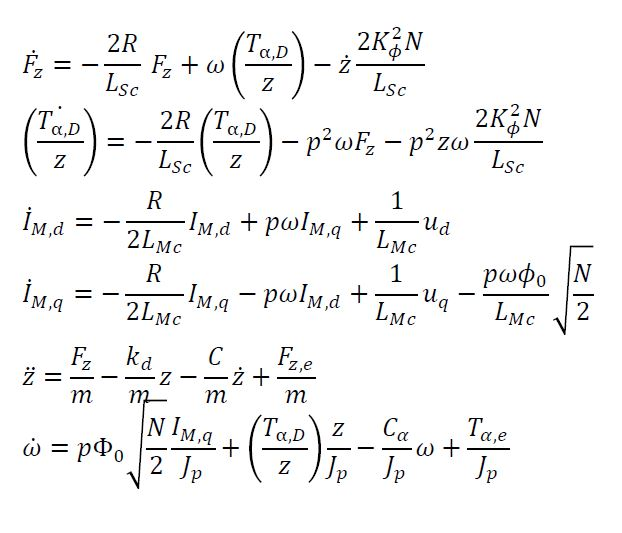
\includegraphics[scale=0.45]{S66.jpg}
    \caption{}
    \label{fig:S66}
\end{figure}

\paragraph{Slide 67} 

Pour la linéarisation, on utilise l'approx de Taylor du premier ordre comme montré sur l'image (Figure \ref{fig:Taylor}). 
\begin{figure}
\centering
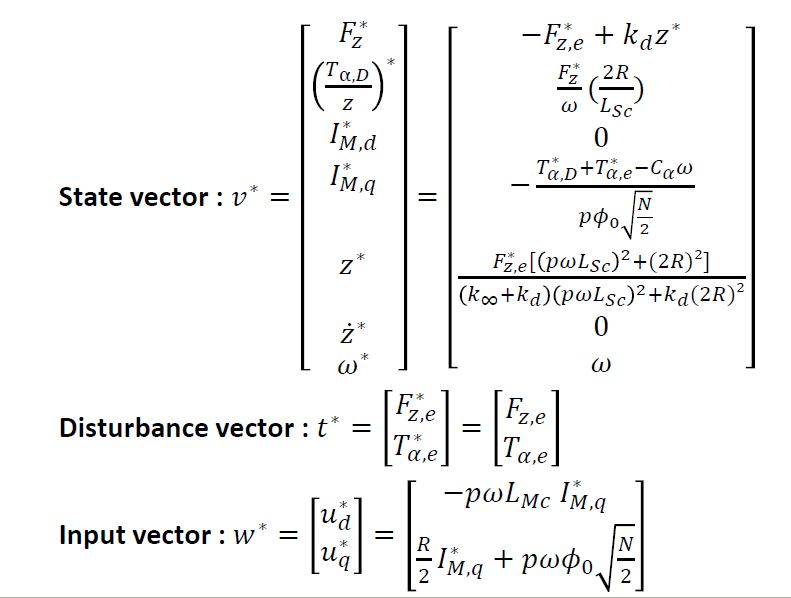
\includegraphics[scale=0.45]{S67.jpg}
\caption{}
\label{fig:S67}
\end{figure}


\begin{figure}[H]
    \centering
    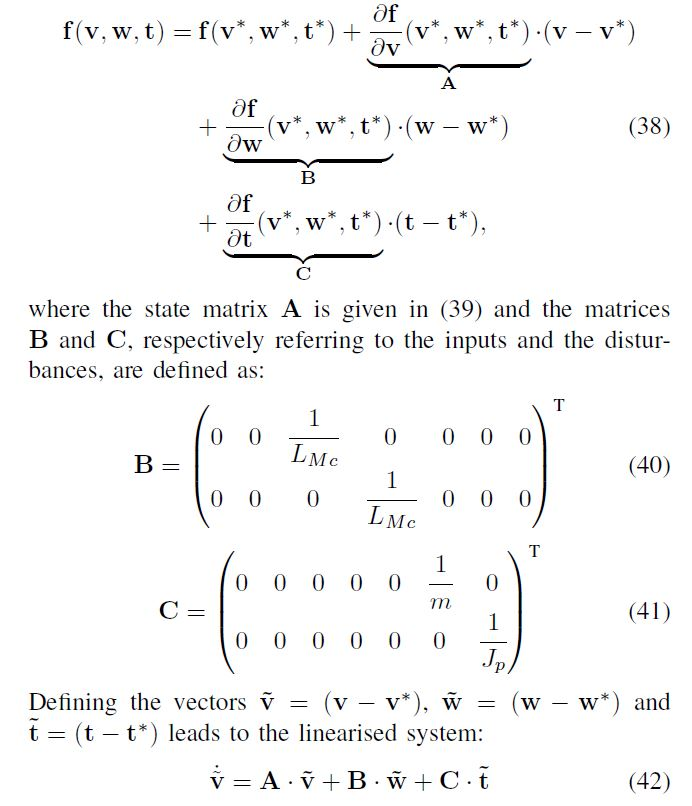
\includegraphics[scale=0.34]{Taylor.JPG}
    \caption{Taylor first order}
    \label{fig:Taylor}
\end{figure}
On doit pour cela définir les 3 vecteurs : vecteur d'état, de perturbations et d'input (voir Figure \ref{fig:S67}).

Le vecteur d'état est défini par les éléments suivants :
\begin{itemize}
    \item La force axiale dynamique fournie par le système (suite à la rotation du rotor), elle est en fait égale à la différence entre la force fournie par les aimants permanents du rotor(donc qui provient du système) et la force ext (provient pas du système)
    \item Le drag torque est le moment qui freine le moteur, c'est un torque qui vient du système. L'expression obtenue pour ce torque est obtenue via la 3ème équation du système 22(3eme équation du système à droite Slide 59) dans le papier mais là encore une fois c'est juste de l'algèbre..
    \item $I_{M,d} = 0$ car la composante directe du courant moteur ne participe pas dans la génération électrodynamique de force ni de torque. En fait cette composante est une source de pertes.
    \item Pour $I_{M,q}$ on voit bien le lien avec les différents couples : Ta,D est le drag torque, Ta,e torque extérieur (freine avec la main) et Ca est le spin additional non-rotating damping. Ce qui est donc important à retenir, c'est que cette composante fournit le torque qui provient du système. Donc la composante quadratique du moteur permet de faire tourner le rotor.
    \item z* est obtenu via de l'algèbre long et chiant. Vient du modèle dynamique
    \item la vitesse axiale est mis à 0 car on linéarise autour d'un point d'équilibre
\end{itemize}

Ensuite le vecteur de perturbations t est juste constitué des forces et torques qui peuvent provenir de l'extérieur -> gravité ou doigt ou quoi.
Finalement le vecteur d'entrée est constitué des deux composantes de la tension qu'on place aux bornes du stator. Les expressions des deux composantes de tensions viennent de l'équation 22 (slide 59) du papier mais encore une fois, c'est juste purement de l'algèbre..

Finalement ce qui nous intéresse vraiment, c'est d'analyser la stabilité via les valeurs propres de A



\paragraph{Slide 68} Voilà les matrices qu'on obtient avec l'approx de Taylor Figure \ref{fig:S68}

\begin{figure}[H]
    \centering
    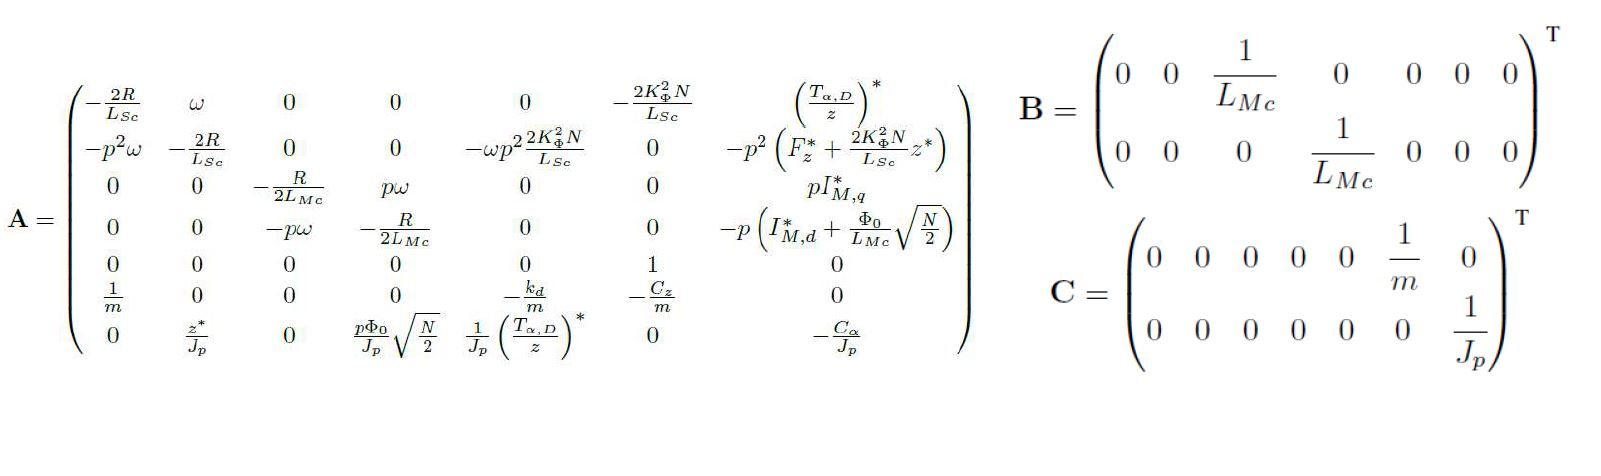
\includegraphics[scale=0.35]{S68.jpg}
    \caption{}
    \label{fig:S68}
\end{figure}




\section{Quasi-Static Analysis}


\paragraph{Slide 69} On voit ici(Figure \ref{fig:S69}) la stiffness totale $k_{t}$, enfait elle est obtenue en faisant la somme de la force dynamique fournie par le système (grâce à la rotation du rotor) et de la force statique fournie par les aimants permanents. Du coup, après on remplace juste Fz/z par son expression (encore une fois juste de l'algèbre). On peut tout de même remarquer une analogie de la forme de Fz avec un circuit RL, ceci est du au fait qu'on a un circuit équivalent RL et que la force axiale fournie est dépendante du courant qui traverse le circuit.
Les trois points importants à retenir sur $k_t$ sont notés sur la droite.




\begin{figure}[H]
    \centering
    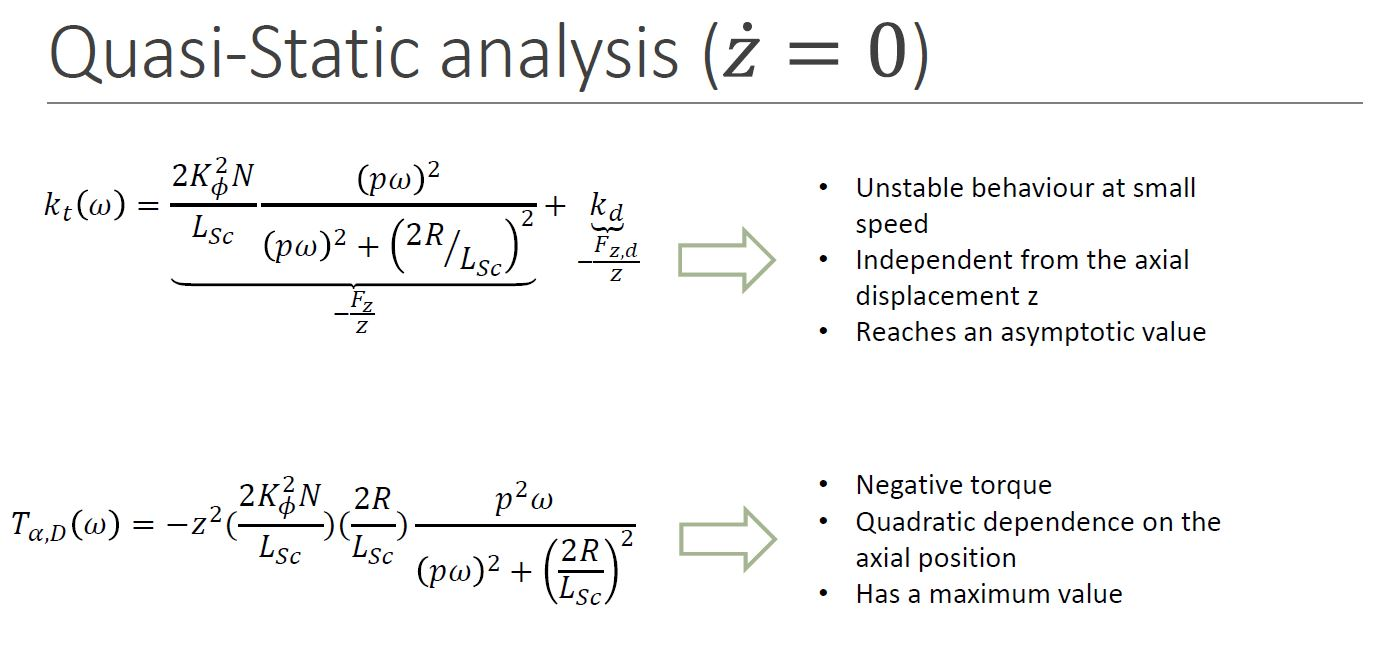
\includegraphics[scale=0.35]{S69.jpg}
    \caption{}
    \label{fig:S69}
\end{figure}


Ensuite on voit l'expression du drag torque, qui est en fait obtenue grâce à l'expression de $\frac{T_{\alpha , D}}{z}$ du slide 67. Les choses importantes à retenir de cette expression sont:
\begin{itemize}
    \item $k_t$
    \begin{itemize}
        \item Comportement instable à basse vitesse
        \item Independant du déplacement axial z
        \item Atteint une valeur asymptotique
    \end{itemize}
    \item $T_{\alpha,D}$
    \begin{itemize}
        \item Torque est négatif
        \item Dépendance quadratique de la position axiale
        \item A une valeure maximale 
    \end{itemize}
\end{itemize}
Cependant, pour ceux qui veulent aller chercher plus loin à quoi est lié physiquement le max du drag torque -> Le max est en $\omega = \frac{2R}{pL_{Sc}}$, on voit donc que c'est lié au pole électrique.

Attention, pour faire cette quasi-static analysis, on a pas encore besoin eu de la linéarisation !

\paragraph{Slide 70} Ici (\ref{fig:S70})on voit bien que la courbe de $k_t$ commence à zéro, c'est en fait parce qu'on a considéré que $k_d$ valait 0.
\begin{figure}[H]
    \centering
    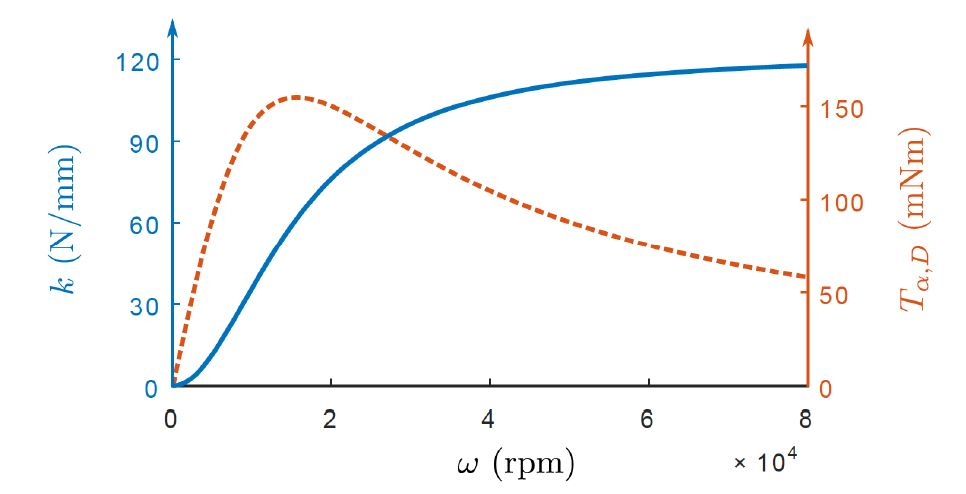
\includegraphics[scale=0.45]{S70.jpg}
    \caption{}
    \label{fig:S70}
\end{figure}
\paragraph{Slide 71} On voit sur la Figure \ref{fig:S71} l'impact de $k_d$ sur $k_t$, si $k_t$ est non nul, on voit bien que ça peut introduire une instabilité STATIQUE à basse vitesse. En effet, si $k_t$ est négatif, la formule $F = -kx$ nous montre que si notre déplacement est positif, la force sera positive aussi, donc au plus le rotor s'éloigne, au plus la force est grande pour qu'il s'éloigne encore plus!
\begin{figure}[H]
    \centering
    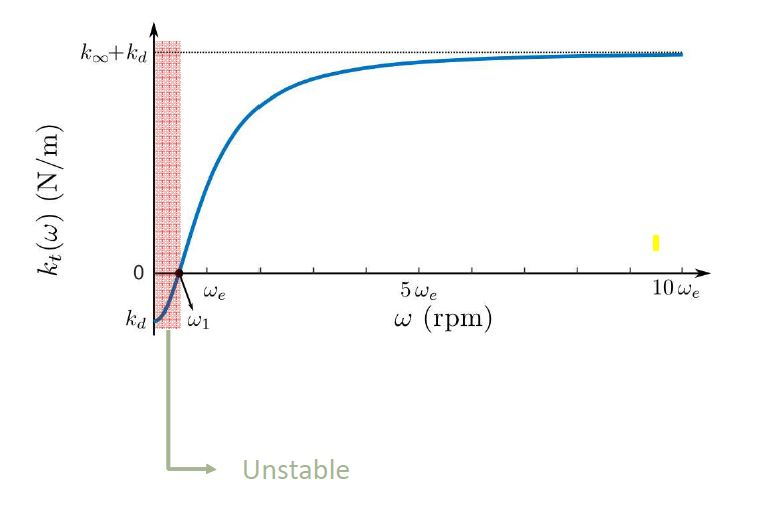
\includegraphics[scale=0.45]{S71.jpg}
    \caption{}
    \label{fig:S71}
\end{figure}

\paragraph{Slide 72} Ici on va déterminer les paramètres de notre système :

\begin{itemize}
    \item Nombre de paires de pole déterminé en fonction du design qu'on souhaite
    \item Résistance du bobinage R, masse du rotor m et le moment polaire $J_p$ sont trouvés grâce à des formules analytiques
    \item Inductances cycliques $L_{Sc}$ et $L_{Mc}$, la raideur axiale de détente $k_d$, la constante de flux $\phi_0$ et le gradient de flux $L_\phi$ sont déterminés grâce à des simulations d'éléments finis
    \item Damping externe axial $C_z$ et damping externe rotationnel $C_\alpha$ sont déterminés par la structure du moteur
\end{itemize}
\section{Stability analysis}
Ici on va utiliser la linéarisation introduite plus tôt !
\paragraph{Slide 74} Rappel Root locus pour ceux qui veulent : https://www.youtube.com/watch?v=CRvVDoQJjYI . Les pôles ici sont obtenus grâce à la matrice A introduite quelques slides plus tôt ! Attention, ici on va parler d'instabilité DYNAMIQUE et non plus statique !! 

Tout d'abord sur le graphe à gauche de la Figure \ref{fig:S74}, on remarque qu'on a 7 courbes différentes(chacune a une couleur différente). On remarque qu'on a 4 pôles stables à gauche, ceux-ci proviennent des équations électriques du système. Les parties réelles des pôles tendents donc vers les constantes du circuit électrique.

\begin{figure}[H]
    \centering
    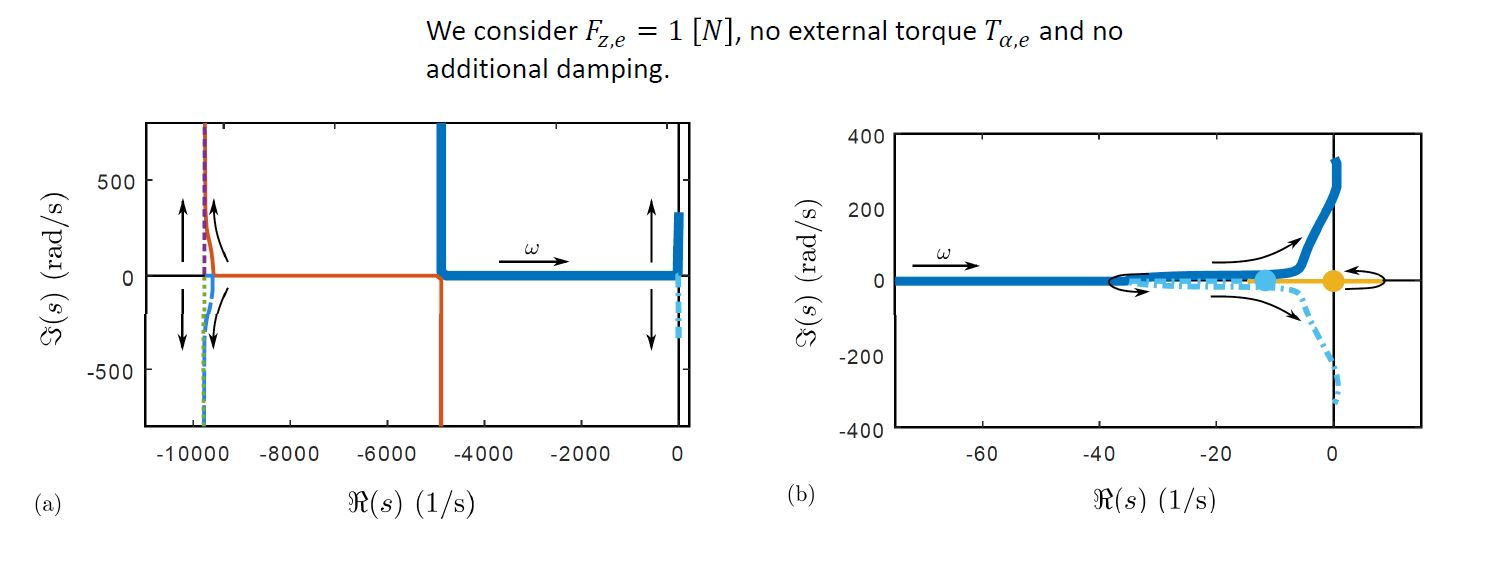
\includegraphics[scale=0.3]{S74.jpg}
    \caption{}
    \label{fig:S74}
\end{figure}

Si on regarde sur le graphe à droite, on voit qu'il y a 3 pôles qui peuvent être instables, ceci est du aux équations mécaniques du système. On peut d'abord voir que quand w=0, on est à la limite de la stabilité pour le pôle en jaune. En suite de 0 à w1, on voit que le jaune sera instable mais pas encore les deux courbes bleues. Ensuite de w1 à w2, le système sera stable. A partir de w2, on aura les deux courbes bleues qui seront instables. 

\paragraph{Slide 75} Ici on a mis les additionnals dampings ratios à zéro ($C_z$ et $C_\alpha$). Sur la figure \ref{fig:S75}, on peut voir la zone de stabilité donc en blanc. La partie hachurée est l'ensemble des pairs de $\omega$ et $F_{z,e}$ qui nous donnerait un déplacement plus grand que ce que notre stator le permet -> donc impossible à avoir un point de fonctionnement pour cette paire. La partie bleue claire marque la zone d'instabilité à haute vitesse et la partie bleue foncée marque la zone d'instabilité à basse vitesse.
On peut aussi remarquer que la zone d'instabilité à basse vitesse dépend quadratiquement de $F_{z,e}$.
\begin{figure}[H]
    \centering
    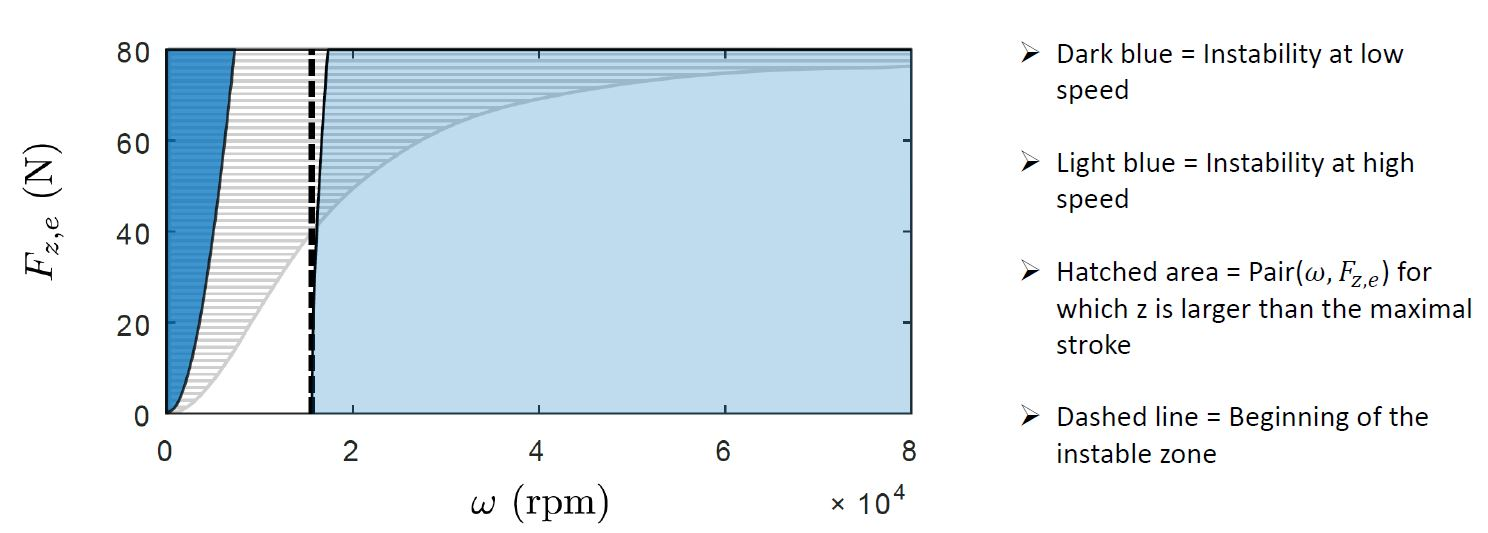
\includegraphics[scale=0.3]{S75.jpg}
    \caption{}
    \label{fig:S75}
\end{figure}

\paragraph{Slide 76} On voit ici ((Figure \ref{fig:S76})) l'impact du axial damping ratio, qui nous permet de réduire la zone d'instabilité à haute vitesse. On peut même faire disparaitre cette zone d'instabilité ! Si on a de très grosses force $F_{z,e}$, on peut passer "au-dessus" de la zone d'instabilité à haute vitesse mais on se retrouvera souvent dans la partie hachurée qui n'est pas accessible physiquement(pour le cas envisagé ici avec une butée bien précise).
\begin{figure}[H]
    \centering
    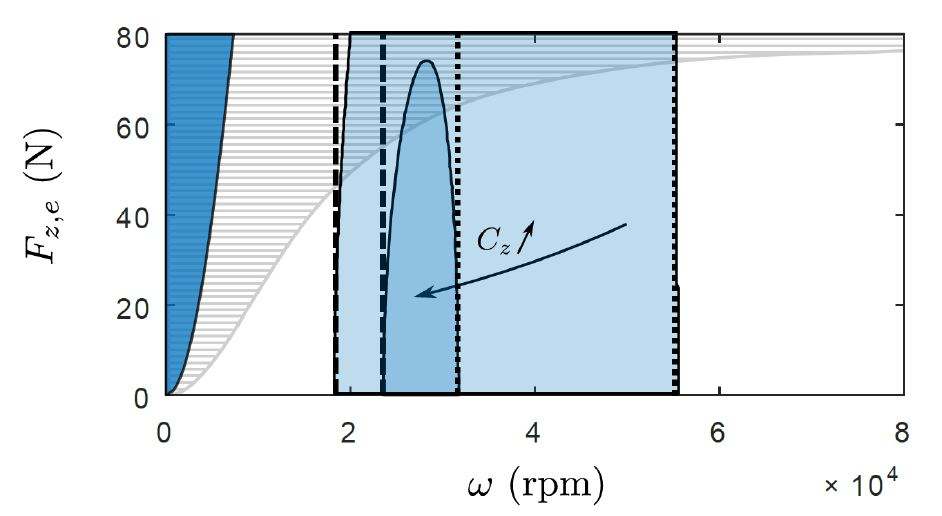
\includegraphics[scale=0.5]{S76.jpg}
    \caption{}
    \label{fig:S76}
\end{figure}
\paragraph{Slide 77} On voit ici (Figure \ref{fig:S77}) l'impact du spin damping ratio sur les deux zones d'instabilité. En augmentant ce ratio, on diminue la zone instable à basse vitesse, par contre, on augmente la zone d'instabilité à grande vitesse.
\begin{figure}[H]
    \centering
    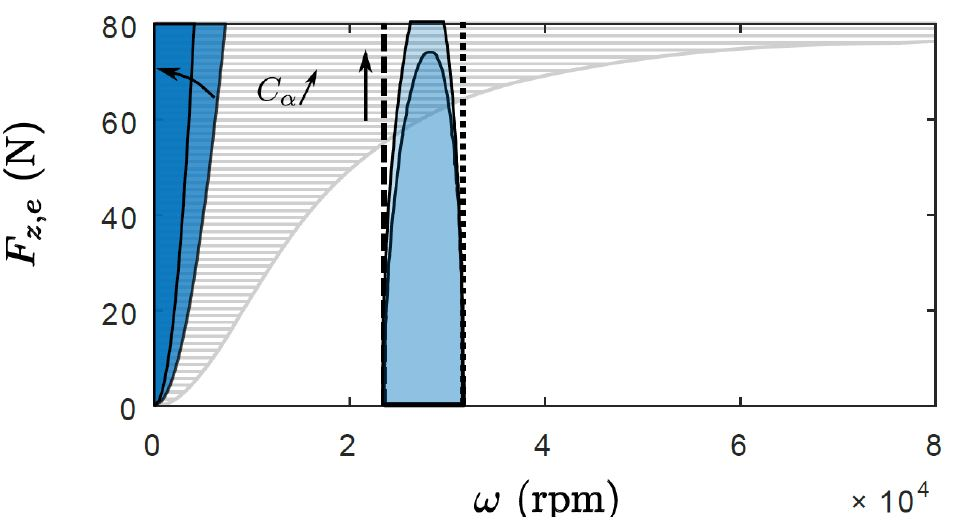
\includegraphics[scale=0.5]{S77.jpg}
    \caption{}
    \label{fig:S77}
\end{figure}





\section{Validation expérimentale - sisi, ça marche}

\paragraph{Slide 80} Controlle classique de notre courant moteur( çela permet juste de fixer notre vitesse de rotation du rotor )   , dans le papier de référence il y a un schéma plus précis mais bruno a dit qu'on s'en fout un peu ;) 

\paragraph{Slide 81} simulation numérique où l'on fixe notre rotor a 4000 RPM et on applique une force externe constante de 1N sur l'axe de notre rotor entre 10 et 20 sec. la ligne bleu représente la force exterieur $F_{z,e}$ et la force de réaction $F_z$ créé par la rotation de notre rotor ( via notre courant de suspension $I_s$). La ligne en pointillé rouge représente la position axial de notre rotor ( avec $z=0$ est la position de lévitation optimal ). on voit qu'un nouveau point d'équilibre est crée a $z=0.13$. Notre courant de suspension va créer, en plus de notre $F_z$, un drag torque parasite qui va s'opposer à la rotation ( en pointillé rouge sur le graphe b ). $I_M$ va produire un torque moteur pour contrer le drag torque

\paragraph{Slide 82} Même principe mais là c'est la force externe qui est cst et c'est le rotor qui accélere grace à $I_M$. notre rotor n'est debase pas a notre position nominal à cause de la force externe, l'accélération va augmenter notre courant passif $I_S$ du coup le rotor se rapproche axialement de notre position nominale. bien faire gaffe que le drag torque est moins important à 6000 RPM qu'à 4000 ( grace à l'augmentation de la rigidité axial $k(\omega)$

\paragraph{Slide 83} Jolie prototype créer par JOJO, 1 = les partie en plastique blanc, 2 = les enroulements collé sur chaque partie, 3 = les aimants permanent, attention que notre rotor est formé de 2 set d'aimants permanents avec une partie en métal qu'ils les fixe ensemble (4). 5 = l'arbre. La partie en alluminium sur le stator a juste une utilité pour la rigidité et résistance du prototype ( aucun courant induit ou autre dans cette partie ) 
\paragraph{Slide 84} Ce slide permet juste de dire pourquoi les hypothèses utilisé au début sont confirmé dans ce prototype ( en parenthèse à chauque point). la 1 c'est juste que le domaine d'application de ce prototype n'est pas propice a de grand déplacement axial ( exemple : dans l'espace ). Pour les autres ça me semble clair. 

\paragraph{Slide 85 à 91} Pas grand chose à dire en +.

\paragraph{Slide 92} Pour cette validation expérimentale, l'expérience est divisé en 3 étape. 1 =on accélère le rotor jusque 6000 RPM, 2 = on stabilise la machine, 3 = on débranche notre source de courant $I_M$. L'important a observer c'est que sur le graphe de droite ( position VS vitesse de rotation ), l'accélération ( courbe bleu ) suit exactement la courbe de décélération ( en rouge ). On peut en conclure que notre force de suspension passif ($F_Z$) est bien indépendante de $I_M$ et que notre courant de suspension, $I_S$ est bien produit par la rotation du rotor. On remarque aussi que notre modèle prévoit bien ce qu'il se passe.  

\paragraph{Slide 93} Ici on mesure la rigidité axial expérimentalement avec la même démarche qu'au slide précédent, on accélère, on stabilise, on débranche. On mesure z et $\omega$ et via l'équation qui est sur le slide on trouve k. on répète çela pour plusieurs tilt d'angle différent de notre prototype ( donc des $F_e$ différents). Il n'y a une différence que 3 de \% entre le théorique et l'expérimentale. Notre modèle est confirmé. Ce slide permet aussi de mettre des valeurs sur cette rigidité. 

\subsection{Améliorer la constant de stifness à basse rotation}

\paragraph{Slide 94} Ici on imagine un domaine d'application de notre prototype à basse vitesse (entre 0 et 5000 RPM). On peut rajouter un inducteur en serie sur l'enroulement de chaque phase de notre  prototype. l'equation de notre rigidité est modifier et est représenter sur le slide. Sur le graphe ( Vitesse de rotation VS Rigidité ) on peut voir la nouvelle courbe théorique ainsi que les points expérimentale trouvé de la même manière qu'au slide 93 pour différent Tilt du prototype. cette courbe est comparé avec la courbe théorique du slide précédent ( sans l'inductance ). On remarque une rigidité bien plus importante jusqu'a 4000 RPM, dépasser ce point notre rigidité est moins efficace qu'avant. 

\appendix

\section{Théorème d'Earnshaw}
L'explication développée ici sera intuitive. Pour la démonstration mathématique, nous vous renvoyons à la page Wikipédia anglophone sur le théorème d'Earnshaw \footnote{consultée le 28 Avril 2019}.

Si deux palliers magnétiques sont dans leurs positions d'équilibre, la somme des forces agissants sur les palliers est nulle. Mais si leurs positions relatives changent, une force apparaitra de manière similaire à des aimants : $F = -kx$. Où k est la constante de raideur, comme dans un ressort.

Le théorème d'Earnshaw prouve qu'il est impossible de stabiliser 6 degrés de libertés en utilisant que des champs magnétiques statiques (matériaux ferromagnétiques ou aimants permanents) car parmis les constantes de raideurs dans les 3 directions, une sera toujours négative. 

Qu'est-ce que cela implique ?
Comme $F = -kx$, si $k < 0$, un déplacement dans une direction entraine une force dans la même direction. Ce qui rend la position initiale (à l'équilibre) instable face à la moindre perturbation.

\begin{figure}[htb!]
    \centering
    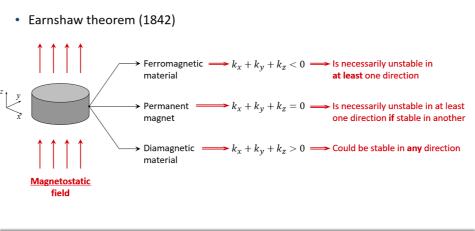
\includegraphics[scale=0.6]{Damon/Earnshaw.png}
    \caption{Théorème d'Earnshaw illustré. }
    \label{fig:Earnshaw}
\end{figure}

Un exemple est repris sur la figure Fig \ref{fig:Passif} : les degrés de libertés axial et de tilt sont stables (la constante de raideur est positive dans ces directions). Mais le degrés de liberté radial est instable : on voit que si la pièce central se rapproche de l'armature, l'interaction Nord-Nord aura tendance à les rapprocher d'autant plus ($F = -kx$ avec $k<0$)

\begin{figure}[htb!]
    \centering
    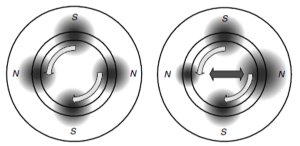
\includegraphics[scale = 0.5]{Damon/PallierPassif.png}
    \caption{Exemple d'un pallier magnétique passif qui stabilise les degrés de libertés axial et de "tilt". Mais le degré de liberté radial est instable.}
    \label{fig:Passif}
\end{figure}
\unappendix
